%% 
%% Copyright 2007-2020 Elsevier Ltd
%% 
%% This file is part of the 'Elsarticle Bundle'.
%% ---------------------------------------------
%% 
%% It may be distributed under the conditions of the LaTeX Project Public
%% License, either version 1.2 of this license or (at your option) any
%% later version.  The latest version of this license is in
%%    http://www.latex-project.org/lppl.txt
%% and version 1.2 or later is part of all distributions of LaTeX
%% version 1999/12/01 or later.
%% 
%% The list of all files belonging to the 'Elsarticle Bundle' is
%% given in the file `manifest.txt'.
%% 

%% Template article for Elsevier's document class `elsarticle'
%% with numbered style bibliographic references
%% SP 2008/03/01
%%
%% 
%%
%% $Id: elsarticle-template-num.tex 190 2020-11-23 11:12:32Z rishi $
%%
%%
\documentclass[preprint,12pt]{elsarticle}

%% Use the option review to obtain double line spacing
%% \documentclass[authoryear,preprint,review,12pt]{elsarticle}

%% Use the options 1p,twocolumn; 3p; 3p,twocolumn; 5p; or 5p,twocolumn
%% for a journal layout:
%% \documentclass[final,1p,times]{elsarticle}
%% \documentclass[final,1p,times,twocolumn]{elsarticle}
%% \documentclass[final,3p,times]{elsarticle}
%% \documentclass[final,3p,times,twocolumn]{elsarticle}
%% \documentclass[final,5p,times]{elsarticle}
%% \documentclass[final,5p,times,twocolumn]{elsarticle}

%% For including figures, graphicx.sty has been loaded in
%% elsarticle.cls. If you prefer to use the old commands
%% please give \usepackage{epsfig}

%% The amssymb package provides various useful mathematical symbols
\usepackage{amssymb, amsmath}
%% The amsthm package provides extended theorem environments
%% \usepackage{amsthm}

%% The lineno packages adds line numbers. Start line numbering with
%% \begin{linenumbers}, end it with \end{linenumbers}. Or switch it on
%% for the whole article with \linenumbers.
%% \usepackage{lineno}

\journal{Computer Physics Communications}

\begin{document}

\begin{frontmatter}

%% Title, authors and addresses

%% use the tnoteref command within \title for footnotes;
%% use the tnotetext command for theassociated footnote;
%% use the fnref command within \author or \address for footnotes;
%% use the fntext command for theassociated footnote;
%% use the corref command within \author for corresponding author footnotes;
%% use the cortext command for theassociated footnote;
%% use the ead command for the email address,
%% and the form \ead[url] for the home page:
%% \title{Title\tnoteref{label1}}
%% \tnotetext[label1]{}
%% \author{Name\corref{cor1}\fnref{label2}}
%% \ead{email address}
%% \ead[url]{home page}
%% \fntext[label2]{}
%% \cortext[cor1]{}
%% \affiliation{organization={},
%%             addressline={},
%%             city={},
%%             postcode={},
%%             state={},
%%             country={}}
%% \fntext[label3]{}

\title{Slepians.jl: A Julia package to generate optimal functions which are 
simultaneously constrained in space and spectral domains}

%% use optional labels to link authors explicitly to addresses:
%% \author[label1,label2]{}
%% \affiliation[label1]{organization={},
%%             addressline={},
%%             city={},
%%             postcode={},
%%             state={},
%%             country={}}
%%
%% \affiliation[label2]{organization={},
%%             addressline={},
%%             city={},
%%             postcode={},
%%             state={},
%%             country={}}

\author[anlmcs]{Charlotte L. Haley}

\author[anlmcs]{M. Anitescu}

\author[anlmcs]{V. Rao}

\author[anlaps]{M. Krogstad}

\author[anlmsd]{R. Osborn}

\author[anlmsd]{S. Rosenkranz}

\affiliation[anlmcs]{organization={Argonne National Laboratory},%Department and Organization
            addressline={Division of Mathematics and Computer Science}, 
            city={Lemont},
            postcode={60439}, 
            state={IL},
            country={USA}}

\affiliation[anlaps]{organization={Argonne National Laboratory},%Department and Organization
            addressline={Advanced Photon Source}, 
            city={Lemont},
            postcode={60439}, 
            state={IL},
            country={USA}}
            
\affiliation[anlmsd]{organization={Argonne National Laboratory},%Department and Organization
            addressline={Materials Science Division}, 
            city={Lemont},
            postcode={60439}, 
            state={IL},
            country={USA}}

\begin{abstract}

In a series of six landmark papers of Slepian, Landau, and Pollak, a set of functions
are described which solve what is known as the ``concentration problem". The
concentration problem refers to finding the subspace of functions having limited support in,
say, time, which simultaneously have a Fourier transform for which the bulk of
its nonzero mass in a small constrained interval. While in some special discrete
cases, it is possible to solve a simple, possibly tridiagonal or Toeplitz eigenvalue 
problem, in others it is necessary
to use numerical integration to solve the defining Fredholm integral equation of the second kind. 
This package produces function values where the problem
dimension is up to three. We rely on the work of Simons, Wang,
\cite{SimonsWang2011} and others, for the two dimensional case but to our knowledge the
three dimensional case is novel to this package. In addition, we implement the
missing data Slepian sequences of Chave \cite{chave2019multitaper} as well as the generalized Slepian
sequences of Bronez \cite{bronez88} which solve the 2D concentration problem on an
unequally spaced spatial grid. We give a novel real data application of these functions to the analysis of the 
pair distribution function, which summarizes the probability of the relative positions of pairs of atoms in a crystal lattice, and is the Fourier transform of the single crystal x-ray scattering (which is understood to be like the spectrum of an unobserved process). 

The companion package to this work represents enhanced computational efficiency above and beyond that which is available at present, and can solve problems in 3D, which is entirely novel. 

\end{abstract}

%%Graphical abstract
\begin{graphicalabstract}
%\includegraphics{grabs}
\end{graphicalabstract}

%%Research highlights
\begin{highlights}
\item Research highlight 1
\item Research highlight 2
\end{highlights}

\begin{keyword}
%% keywords here, in the form: keyword \sep keyword

%% PACS codes here, in the form: \PACS code \sep code

%% MSC codes here, in the form: \MSC code \sep code
%% or \MSC[2008] code \sep code (2000 is the default)

\end{keyword}

\end{frontmatter}

%% \linenumbers

%% main text

\section{Introduction}
In the early 1960s, the prolate spheroidal wave functions (pswf) of Slepian, Landau, and Pollak \cite{pswf1,pswf2,pswf3,pswf4} were a series of landmark papers published
in the Bell System Technical Journal which described a special one-dimensional class of functions 
having finite extent in time but constrained extent in the spectral (or frequency) domain. 

One of the earliest applied contributions making use of these functions was the multitaper method of Thomson \cite{T82, pw93} which, 
simply put, used the discrete analog of the pswfs, \cite{S78}, as data windows to constrain spectral leakage and reduce variance when estimating quantities in the spectral domain such as the power spectrum, coherency, and so forth. While the multitaper estimator introduces a moderate amount of localized bias, the reduction in far-field bias and variance can be shown to be large, so much so that in comparsion with Welch spectrum estimators, when two of bias, variance, and bandwidth are kept constant, it can be shown \cite{bronez92} that the third quantity is always smaller when one employs the multitaper spectrum estimator. 

The pwsfs $g(x)$ solve the concentration problem in which a bandlimited signal is optimized in a mean squared sense to live strictly within a predefined interval in time \cite{slepian83}. More generally, one can refer to the problem of constraining the spacelimited function defined over a particular domain of interest, where the space of origin may be Cartesian \cite{simons2011} on the sphere \cite{simons2006} or other. 

\section{Mathematical Preliminaries}

The concentration problem of Slepian, Landau and Pollak, seeks to find bandlimited functions
$g(t)$, i.e. functions satisfying 

\begin{equation} g(t) = \frac{1}{2 \pi} \int_{-W}^{W} G(\omega) e^{i\omega t} d\omega \end{equation}

where $G(\omega)$ denotes the Fourier transform of the function $g(t)$, i.e.

\begin{equation} G(\omega) = \int_{-\infty}^{\infty} f(t) e^{-i\omega t} dt \end{equation}

that maximize the ratio 

\begin{equation} \lambda = \frac{\int_{-T}^{T} g^2(t)dt}{\int_{-\infty}^{\infty} g^2(t)dt}. \end{equation}

$\lambda$ is referred to as the concentration. It was shown that these functions
satisfy the Fredholm integral equation of the second kind

\begin{equation} \int_{-T}^{T} \frac{\sin [W (t - s)]}{\pi (t-s)} g(s)ds = \lambda g(t) \end{equation}

for real $t$. 

\section{Discrete prolate spheroidal sequences}

The discrete prolate spheroidal sequences \cite{S78}, $v_n^{(k)}(N,W)$, are the
discrete analog to the above functions $g(t)$. As such, they are the eigenvector
solutions to the eigenvalue problem

\begin{equation}\label{eq:dpss}
\sum_{m = 0}^{N-1}\frac{\sin 2\pi W(n-m)}{\pi(n-m)}v_m^{(k)}(N,W) = \lambda_k(N,W)\cdot v_n^{(k)}(N,W)
\end{equation}

where $N$ is the length of the sequence, $n = 0, \ldots, N-1$, $W$ is the bandwidth,
$K$ is the number of tapers, and $\lambda_k(N,W)$ is the eigenvalue corresponding to
the $k$th taper. Fig. \ref{fig:dpss} shows the discrete prolate spheroidal sequences
calculated using $N = 1,024$, $NW=4$, and $K=8$. 

\begin{figure} \centering
\begin{tabular}{cc}
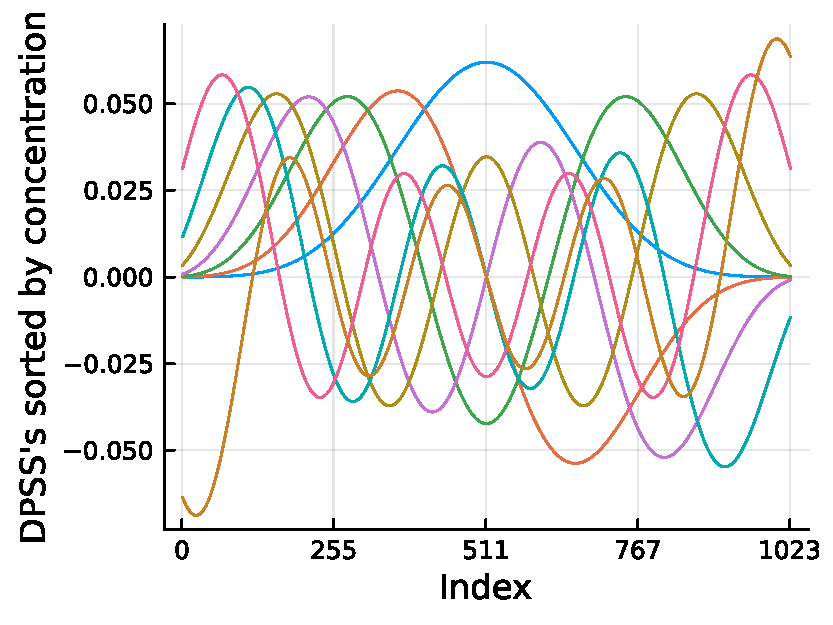
\includegraphics[width=0.45\textwidth]{../figures/Dpss_time.pdf} &
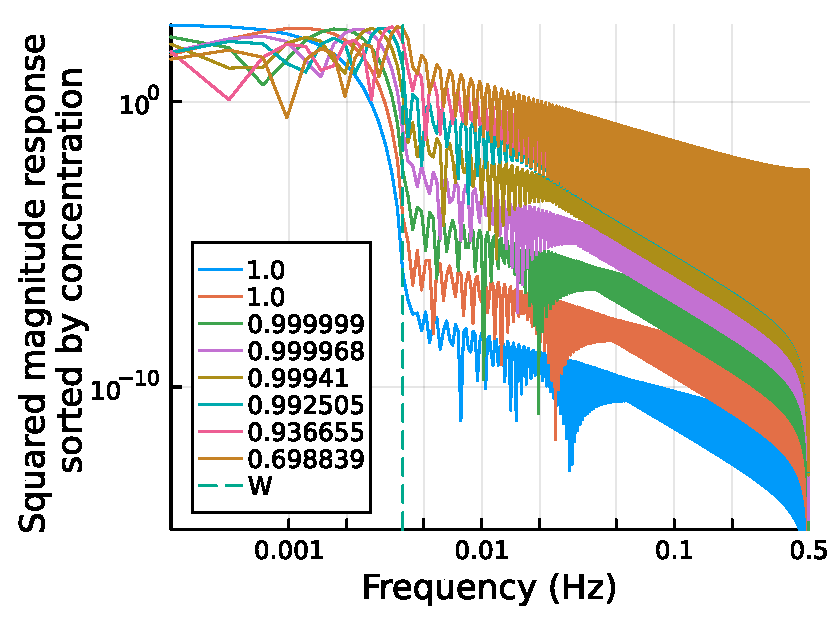
\includegraphics[width=0.45\textwidth]{../figures/Dpss_freq.pdf}
\end{tabular}
\caption{\label{fig:dpss} Standard discrete prolate spheroidal sequences computed
using Eqn. \eqref{eq:dpss} and parameters $N = 1,024$, $NW=4$, and $K=8$. Left panel
shows the sequences in the time domain, while the right panel shows the squared
magnitude of their Fourier transforms. The sequences have their mass (indicated by
the value of $\lambda$ in the legend -- the first two values of $\lambda$ are
$0.9999999997055463, 0.999999972328674, 0.9999987902597943$, which have been rounded
in the legend) concentrated in the
region $(-W,W)$, where $W$ is shown by the vertical line in the right panel.}
\end{figure}

The dpss's solve the problem of concentrating, in frequency, the most amount of mass
under the interval $(-W,W)$, while having only finite extent in time. The first $2NW$
tapers have eigenvalues close to one, whereby their magnitude drops off rapidly
thereafter. 

Of note is that the dpss's are never computed using the above equation because of
numerical instability. Grunbaum \cite{grunbaum81} showed that the associated differential operator
commutes with a symmetric tridiagonal matrix $T$, which is

\begin{equation} T_{nn} = [(N-1-2n)/2]^2 \cos (2\pi W), \quad n = 0, \ldots, N-1\end{equation}

on the diagonal and 

\begin{equation} T_{n, n + 1} = T_{n, n-1} = (n + 1)(N - n - 1)/2, \quad n = 0, \ldots, N-2\end{equation}

on the sub and super diagonals. The matrix $T$ has the same eigenvectors as the
problem above and the eigenvalues can be found by substitution into the original
equation. The tridiagonal formulation reduces the computation to one which is soluble
in O($N$) time, and the solution tends to be more accurate.

Generate a Durrani-Chapman filter \cite{durranic84}

\section{Generalized Prolate Spheroidal Sequences }
 
The missing-data multitaper method requires its own set of optimal tapers
\cite{T82,bronez88,chave2019multitaper}, the \emph{missing-data prolate spheroidal
sequences} or missing-data Slepian sequences. These sequences extend the notion of
maximally bandlimited orthogonal sequences, \cite{S78}, to those sampled on a grid
where there is missing-data.  Define the bandwidth $W$ for the desired spectral
window, and let the sequences be given on the length $N$ index set
$\{t_n\}_{n=0}^{N-1}$ with unit sampling except where there are gaps. 

The missing-data Slepian sequences solve the eigenvalue problem, equations (21)-(23) in \cite{Chave2019},
\begin{equation} \label{eq:mdslep} 
  \lambda_k v^{k}_{n} = \sum_{m=0}^{N-1} \frac{\sin 2\pi W (t_n - t_m) }{\pi (t_n - t_m)} v^{k}_{m}.\end{equation}
The $k$th missing-data Slepian sequence is denoted $v^{k}_{n}$ at time $t_n$, and
and $\lambda_k$ is its associated eigenvalue, sorted in decreasing order
$1>\lambda_0>\lambda_1>\ldots>\lambda_{N-1}>0$. Note that both of these explicitly
depend on $N$ and $W$, but for simplicity this is suppressed in the notation. When
there are no missing values, the sinc-like matrix in (\ref{eq:mdslep}) is
Toeplitz and has a special form which allows for numerically effective eigenvalue
routines.  

By applying the nonuniform discrete Fourier transform to the generalized data taper
in (\ref{eq:mdslep}), one obtains the missing-data prolate spheroidal functions, or
\emph{missing-data Slepian functions}

\begin{equation} V^{k}(f) = \sum_{n = 0}^{N-1} v^{k}_{n} e^{-2 \pi i t_n f}. \end{equation}

The missing-data Slepian sequences form an orthonormal set on the grid
$\{t_n\}_{n=0}^{N-1}$; and the missing-data Slepian functions are orthonormal on
$(-1/2,1/2)$ and orthogonal on $(-W,W)$. 

Show a figure as an example

\section{Higher dimensional Cartesian Slepian functions}

While what follows is contained entirely in \cite{simons2011}, we introduce the mathematical 
preliminaries and establish notation in this section. 

In two dimensions, one can consider the problem of concentrating a function in a region of physical space
for application to data collected from the natural sciences. For this application we are concerned with the 
numerical solution to a Fredholm integral equation of the second kind. 

\section{Examples}

\subsection{One Dimensional Examples}
% Black forest observatory spectral analysis

\subsubsection{Missing data spectral analysis}


\subsection{X-ray Scattering of single crystals}

We give a novel real data application of these functions to the analysis of the 
pair distribution function, which summarizes the probability of the relative positions of pairs of atoms in a crystal lattice, and is the Fourier transform of the single crystal x-ray scattering (which is understood to be like the spectrum of an unobserved process).

\section{Software}

`Slepians.jl` is a Julia package for producing simultaneously time and bandlimited
sequences, as well as space and spectrally limited functions up to three dimensions.
These functions were introduced by Slepian, Landau, and Pollak in the 1960s and have
had particular application in diverse fields, perhaps most notably as foundational
for the multitaper method for spectrum analysis \cite{T82} which extends both to 2D
Cartesian domains \cite{SimonsWang2011} as well as the sphere \cite{simons2006}. 

The high-level character of Julia allows for widely readable and extendible codes,
while the low-level functionality provides speed and efficiency. The `Multitaper.jl`
package provides a user-friendly implementation of many of the basic concepts.
Implementations of higher-dimensional Slepian tapers on Cartesian domains
\cite{SimonsWang2011,Geoga2018}. In addition, we provide tutorial-style notebooks to
allow accessibility to those new to these concepts or to Julia in general.

`Slepians.jl` has been used in the context of 3D pair distribution function analysis
of crystal structure. 

\section{Other software}

The Matlab software of Frederik Simons's research group is available on github under
\texttt{https://github.com/csdms-contrib}, of particular note is \cite{slepian_foxtrot}
which relies on \cite{slepian_alpha} and \cite{slepian_delta}. These packages

\section{To contribute}

We welcome input of any kind via bitbucket issues or by pull requests.
Support requests can kindly be directed to haley@anl.gov.

\section{Acknowledgements}

We acknowledge contributions from David J. Thomson, Sally
Dodson-Robinson during the writing of these codes. We also gratefully acknowledge the
help of our reviewers in editing the code repository.

This work was supported by the U.S. Department of Energy, Office of Science, Advanced
Scientific Computing Research, under contract number DE-AC02-06CH11357.

The submitted manuscript has been created by UChicago Argonne, LLC, Operator of
Argonne National Laboratory (“Argonne”). Argonne, a U.S. Department of Energy Office
of Science laboratory, is operated under Contract No. DE-AC02-06CH11357. The U.S.
Government retains for itself, and others acting on its behalf, a paid-up
nonexclusive, irrevocable worldwide license in said article to reproduce, prepare
derivative works, distribute copies to the public, and perform publicly and display
publicly, by or on behalf of the Government. The Department of Energy will provide
public access to these results of federally sponsored research in accordance with the
DOE Public Access Plan. http://energy.gov/downloads/doe-public-access-plan


%% The Appendices part is started with the command \appendix;
%% appendix sections are then done as normal sections
%% \appendix

%% \section{}
%% \label{}

%% If you have bibdatabase file and want bibtex to generate the
%% bibitems, please use
%%
  \bibliographystyle{elsarticle-num} 
  \bibliography{../paper.bib,../../../../Collected.bib}

%% else use the following coding to input the bibitems directly in the
%% TeX file.
%
%\begin{thebibliography}{00}
%
%%% \bibitem{label}
%%% Text of bibliographic item
%
%\bibitem{}

%\end{thebibliography}
\end{document}
\endinput
%%
%% End of file `elsarticle-template-num.tex'.
